This chapter introduces modeling and design details of Sangamon reactors:  the Sangamon200, and a scaled-down version, the Sangamon20; inspired by the pebble bed designs of the PBMR \cite{venter_pbmr_2005, noauthor_pebble_2017}, Xe-100 \cite{harlan_ans_2017, harlan_x-energy_2018}, and the smaller size of the HTR-10.  Both Sangamon200 and Sangamon20 are UCO-pebble fueled, helium cooled reactors.  All simulations used Serpent version 2 \cite{leppanenjaakko_serpent_2015} with postprocessing and analysis performed using Python \cite{van_rossum_python_nodate} and the Python libraries numpy \cite{harris_array_2020} and PyNE \cite{scopatz_pyne:_2012}.

Before one can confidently analyze reactor physics and safety, it is important to ensure the models used are reliably defined and well-understood.  To this end, \autoref{sec:dispersal} and \autoref{sec-run-params} will lay the foundation for the model, describing mechanics of the particle dispersal routine and the Monte Carlo run parameters.  The following sections, \autoref{meth-burn} and \autoref{meth-comp}, detail the single-pebble models, which are used to find the fuel compositions used in the full-core models.  The full-core models themselves are described in \autoref{s200} and \autoref{s20}.  Finally, the last sections of this chapter detail the various effects we test by perturbing the Sangamon20 model.

\section{Modeling Particle and Pebble Dispersal}
\label{sec:dispersal}

Often in HTGR modeling, a uniform lattice is used to approximate the locations of TRISO particles and fuel pebbles.  However, this doesn't reflect realistic TRISO distributions in the pebbles and pebble distribution in the core.  Pebbles are not perfectly stacked in the core.  Further, models utilizing lattices often cut off portions of pebbles at the boundaries that don't perfectly fit.  Instead, the Sangamon200 and Sangamon20 use a random placement of pebbles.  This random dispersal is not only truer to a real pebble-bed, but restricts pebble locations to the boundaries of the core, ensuring edge effects are accounted for in our models.

In order to determine the locations of random TRISO particles and pebbles, the Serpent particle dispersal routine was leveraged.  The routine takes either the number of particles, defined by the user; or $\eta_{pf}$, the packing fraction (the total volume of particles divided by the volume of that space).  The user must define the particle radius, and the size and shape of the volume housing the particles.  The routine first randomly determines a single point for each particle contained in the volume.  Then, the routine uses the 'growth factor' and 'shake factor' - both described as fractions of the particle radius, and iterates.  During each iteration, the size of the point's radius increases by the growth factor.  Additionally, the center will move in a random direction a distance equal to the shake factor.  If the particle growth causes the particle to overlap with another particle or leave the volume, it doesn't grow that cycle.  Similarly, if the center's movement causes overlap or the particle to leave the containing volume, it doesn't move \cite{cole_gentry_generate_2015}.  The dispersal routine iterates until all particles are to their full size, contained in the volume, and not overlapping with any other particles.  The routine generates an output file, in which each line gives the location of a particle center (in x,y,z coordinates), a particle radius, and the name of the particle type, to associate it with the "pbed" (short for pebble bed) card (see the input syntax manual from \cite{leppanenjaakko_serpent_2015}).  For this work, we used a growth factor of 0.05 and a shake factor of 0.1 \cite{cole_gentry_generate_2015}.

\section{Run Parameters and Conditions}
\label{sec-run-params}

All Serpent 2 simulations and post-processing scripts were run on an Ubuntu 18.04 machine using Python version 3.8.5, numpy version 1.19.2, and PyNe version 0.7.1.  Cross-section data is from the JEFF 3.1.2 data libraries.  Below, Table \ref{table:run-params} gives the Monte Carlo run parameters for each Serpent model.

\begin{table}[h!]
\centering
\caption{Relevant Monte Carlo Parameters for Single Pebble and Sangamon Reactor Simulations}
\begin{tabular}{ c  c  c  c }
\hline
Parameter & Single Pebble & Sangamon200 & Sangamon20 \\
\hline
Active Cycles & 500 & 150 & 100 \\
Inactive Cycles & 250 & 50 & 50  \\
Neutron Population & 20000 & 70000 & 50000 \\
\hline
\end{tabular}

\label{table:run-params}
\end{table}

All input files are available on github at \cite{richter_zoerichterphlox_2022}.

\section{Single Pebble Depletion Model Geometry and Materials}
\label{meth-burn}
The single pebbles are the only simulations that utilize individually defined TRISO particles by default.  Each pebble has an inner region containing the TRISO particles embedded in graphite, and an outer region consisting only of graphite as illustrated by Figure \ref{fig:pebb-zone1}.

\begin{table}[h!]
\centering
\caption{Relevant Material Properties Used in Monte Carlo Simulations}
\begin{tabular}{ c  c  c }
\hline
Material & Denisity $[\frac{g}{cc}]$ & Source \\
\hline
UCO & 11.0 & \cite{helmreich_year_2017, nagley_fabrication_2010}  \\
Graphite & 1.74 & \cite{ho_graphite_1988, johnson_properties_1976} \\
Pyrolytic Carbon & 2.20 & \cite{espi_metals_graphite-pyrolytic_2019} \\
Silicon Carbide & 3.10 & \cite{accuratus_silicon_2013} \\
\hline
\end{tabular}

\label{table:mat-params}
\end{table}

Table \ref{table:mat-params} above give the densities of all solid materials in the model.  The density of the helium coolant was calculated using the ideal gas law \cite{levine_derivation_nodate}.  The graphite reflector properties are assumed to be the same as the buffer layer in TRISO particles (which is assumed to have the same properties as the graphite matrix in the pebbles).

\begin{figure}[H]
\centering


\includegraphics[width=0.5\linewidth]{figures/pebble-zones.png}
\caption{Pebble Zones}
\label{fig:pebb-zone1}
\end{figure}


\begin{table}[h!]
\centering

\caption{Pebble Parameters}
\begin{tabular}{ c  c }
\hline
Parameter & Value \\
\hline
Fueled-Center Radius [cm] & 2.5 \\
Graphite Outer Shell Thickness [cm] & 0.5 \\
Total Radius [cm] & 3.0 \\
TRISO Particles per Pebble & 18,000 \\
\hline
\end{tabular}
\label{table:peb-params}
\end{table}


Above, Figure \ref{fig:pebb-zone1} shows the fueled vs non-fueled regions of the pebbles, while Table \ref{table:peb-params} provides the geometric measurements of the pebbles.  For homogenized pebbles, the "fuel zone" is the homogenized center consisting of dispersed TRISO particle material blended with graphite, while the non-fueled region is pure graphite.  Each region homogenized by volume fraction uses the "mix" card (see \cite{leppanenjaakko_serpent_2015}) in Serpent to blend the fuel, TRISO layer, and graphite matrix materials.  In heterogenized models, the fueled region marks the part of the pebble where TRISO particles are located inside a graphite matrix, and the non-fuel region is the area of pure graphite that surrounds it.  Below, Figure \ref{fig:particle-layer} and Table \ref{table:particle-params} give detailed measurements on geometric dimensions of a TRISO particle and its layers, and gives a visual reference.  Figures \ref{fig:particle-layer} and \ref{fig:pebb-zone1} are both to scale.


\begin{figure}[H]
\centering

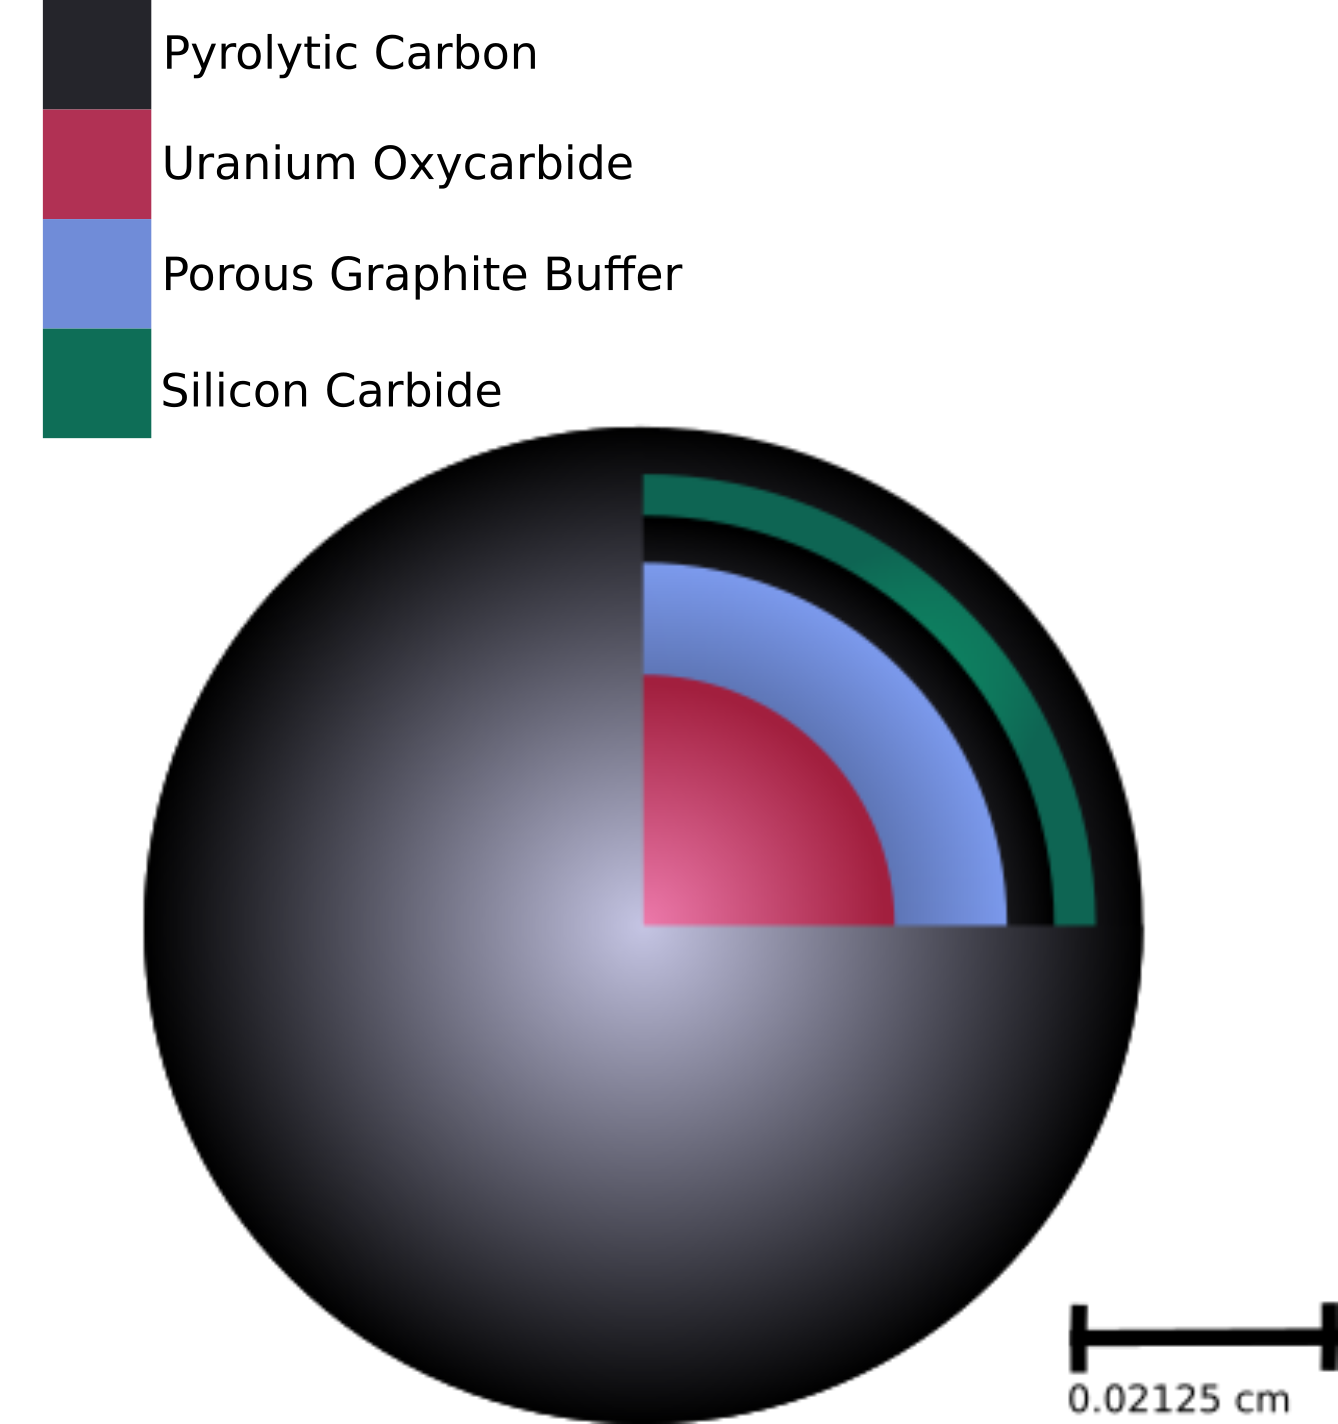
\includegraphics[width=0.5\linewidth]{figures/trisos-r-like-onions.png}
\caption{TRISO Particle Layers}
\label{fig:particle-layer}
\end{figure}

\begin{table}[h!]
\centering

\caption{Particle Parameters Used in Monte Carlo Simulations}
\begin{tabular}{ c  c }
\hline
Parameter & Value [cm] \\
\hline 
Uranium Oxycarbide Kernel Radius & 0.02125 \\
Graphite Layer Thickness & 0.03075 \\
Inner Pyrolytic Carbon Layer Thickness & 0.03475 \\
Silicon Carbide Layer Thickness & 0.03825 \\
Outer Pyrolytic Carbon Layer Thickness & 0.04225 \\
\hline
\end{tabular}
\label{table:particle-params}

\end{table}


\subsection{Fuel Composition Determination}
\label{meth-comp}

The residence time of a pebble in the active core determines its isotopic composition.  We chose to model seven possible pebble compositions, one for each of the six 6-month passes, plus an additional composition for fresh pebbles.  The seven pebble compositions are equally and randomly distributed in the core.

The design approximates the exact isotopic composition by running a burnup calculation using Serpent for a single pebble inscribed within a cube of helium.  The model uses a reflective boundary condition, and burnup steps are measured in days, with each step corresponding to a complete six-month pass: 180, 360, 540, 720, 900, and 1080 days.

\begin{figure}[H]
\centering
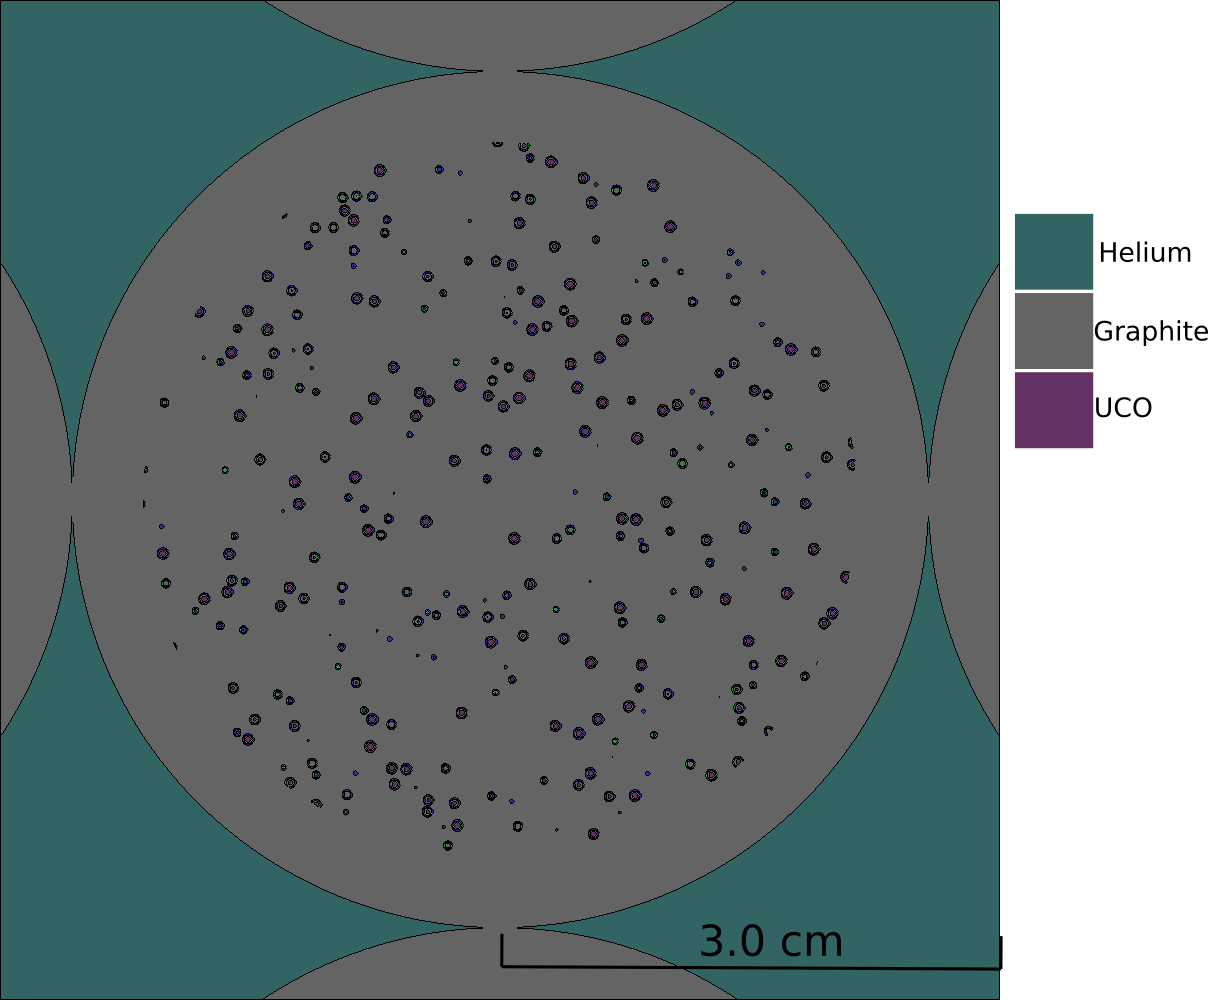
\includegraphics[width = 10cm]{figures/burn-20.png}
\caption{Geometry of the Single-Pebble Burnup Calculation for Sangamon20}
\label{fig:burn-20}
\end{figure}

Figure \ref{fig:burn-20} is a cross-sectional slice of the pebble used in the depletion runs performed by Serpent.  With seven depletion states in total --- one for each pass, plus one for the fresh fuel --- we subsequently have seven unique pebble compositions.  Both the Sangamon20 and Sangamon200 models use this method to generate the necessary isotopic compositions, though they have a different starting enrichment (see \ref{table:params1} in the fresh pebbles.


\section{Sangamon200}
\label{s200}
The top and bottom of the reactor core are a flat surface, to create a cylindrical shape for the active core.  The graphite reflector, which is a cylindrical shell as well, surrounds it with no barriers between the reflector and active core region. There are no control rods included in these simulations.

\begin{table}[h!]
\centering
\caption{Geometric and Internal Core Parameters in the Sangamon Reactors}
\begin{tabular}{ c  c  c }
\hline
Parameter & Sangamon200 \cite{harlan_x-energy_2018}, \cite{harlan_ans_2017} & Sangamon20 \\
\hline
Thermal Power [MW] & 200 & 20 \\
Average Core Temperature [K] & 800 & 800 \\
Enrichment [wt\%] & 15.5\% & 19.75\% \\
Average Core Pressure [MPa] & 5.9 & 5.9 \\
Outer Core Radius [cm] & 216 & 165 \\
Outer Core Height [cm] & 1150 & 330 \\
Reflector Thickness [cm] & 92 & 75 \\
Number of Pebbles & 220,000 & 22,680 \\
Packing Fraction [\%] & 53.0 & 56.0 \\
\hline
\end{tabular}

\label{table:params1}
\end{table}

While Sangamon200 is not the focus of this assessment, some parameters were used to develop the Sangamon20's design.  We used the outward current of the reflector to constrain the Sangamon20 design such that the external exposure of the 20 MWth design was less than or equal to the 200 MWth design.  To do so, a surface detector placed in the reflector, just inside the outer bound of the reflector, shown in Figure \ref{fig:det-place}, to tally the outward neutron current.  When determining the appropriate reflector thickness in Sangamon20, this current is used as an upper boundary and reference point --- that is, the graphite reflector must not only be sufficient to keep the reactor critical, but must also keep the outward surface current less than or equal to Sangamon200's to protect the \acrshort{rpv}.

\begin{figure}[H]
\centering
\resizebox{0.5\textwidth}{!}{%
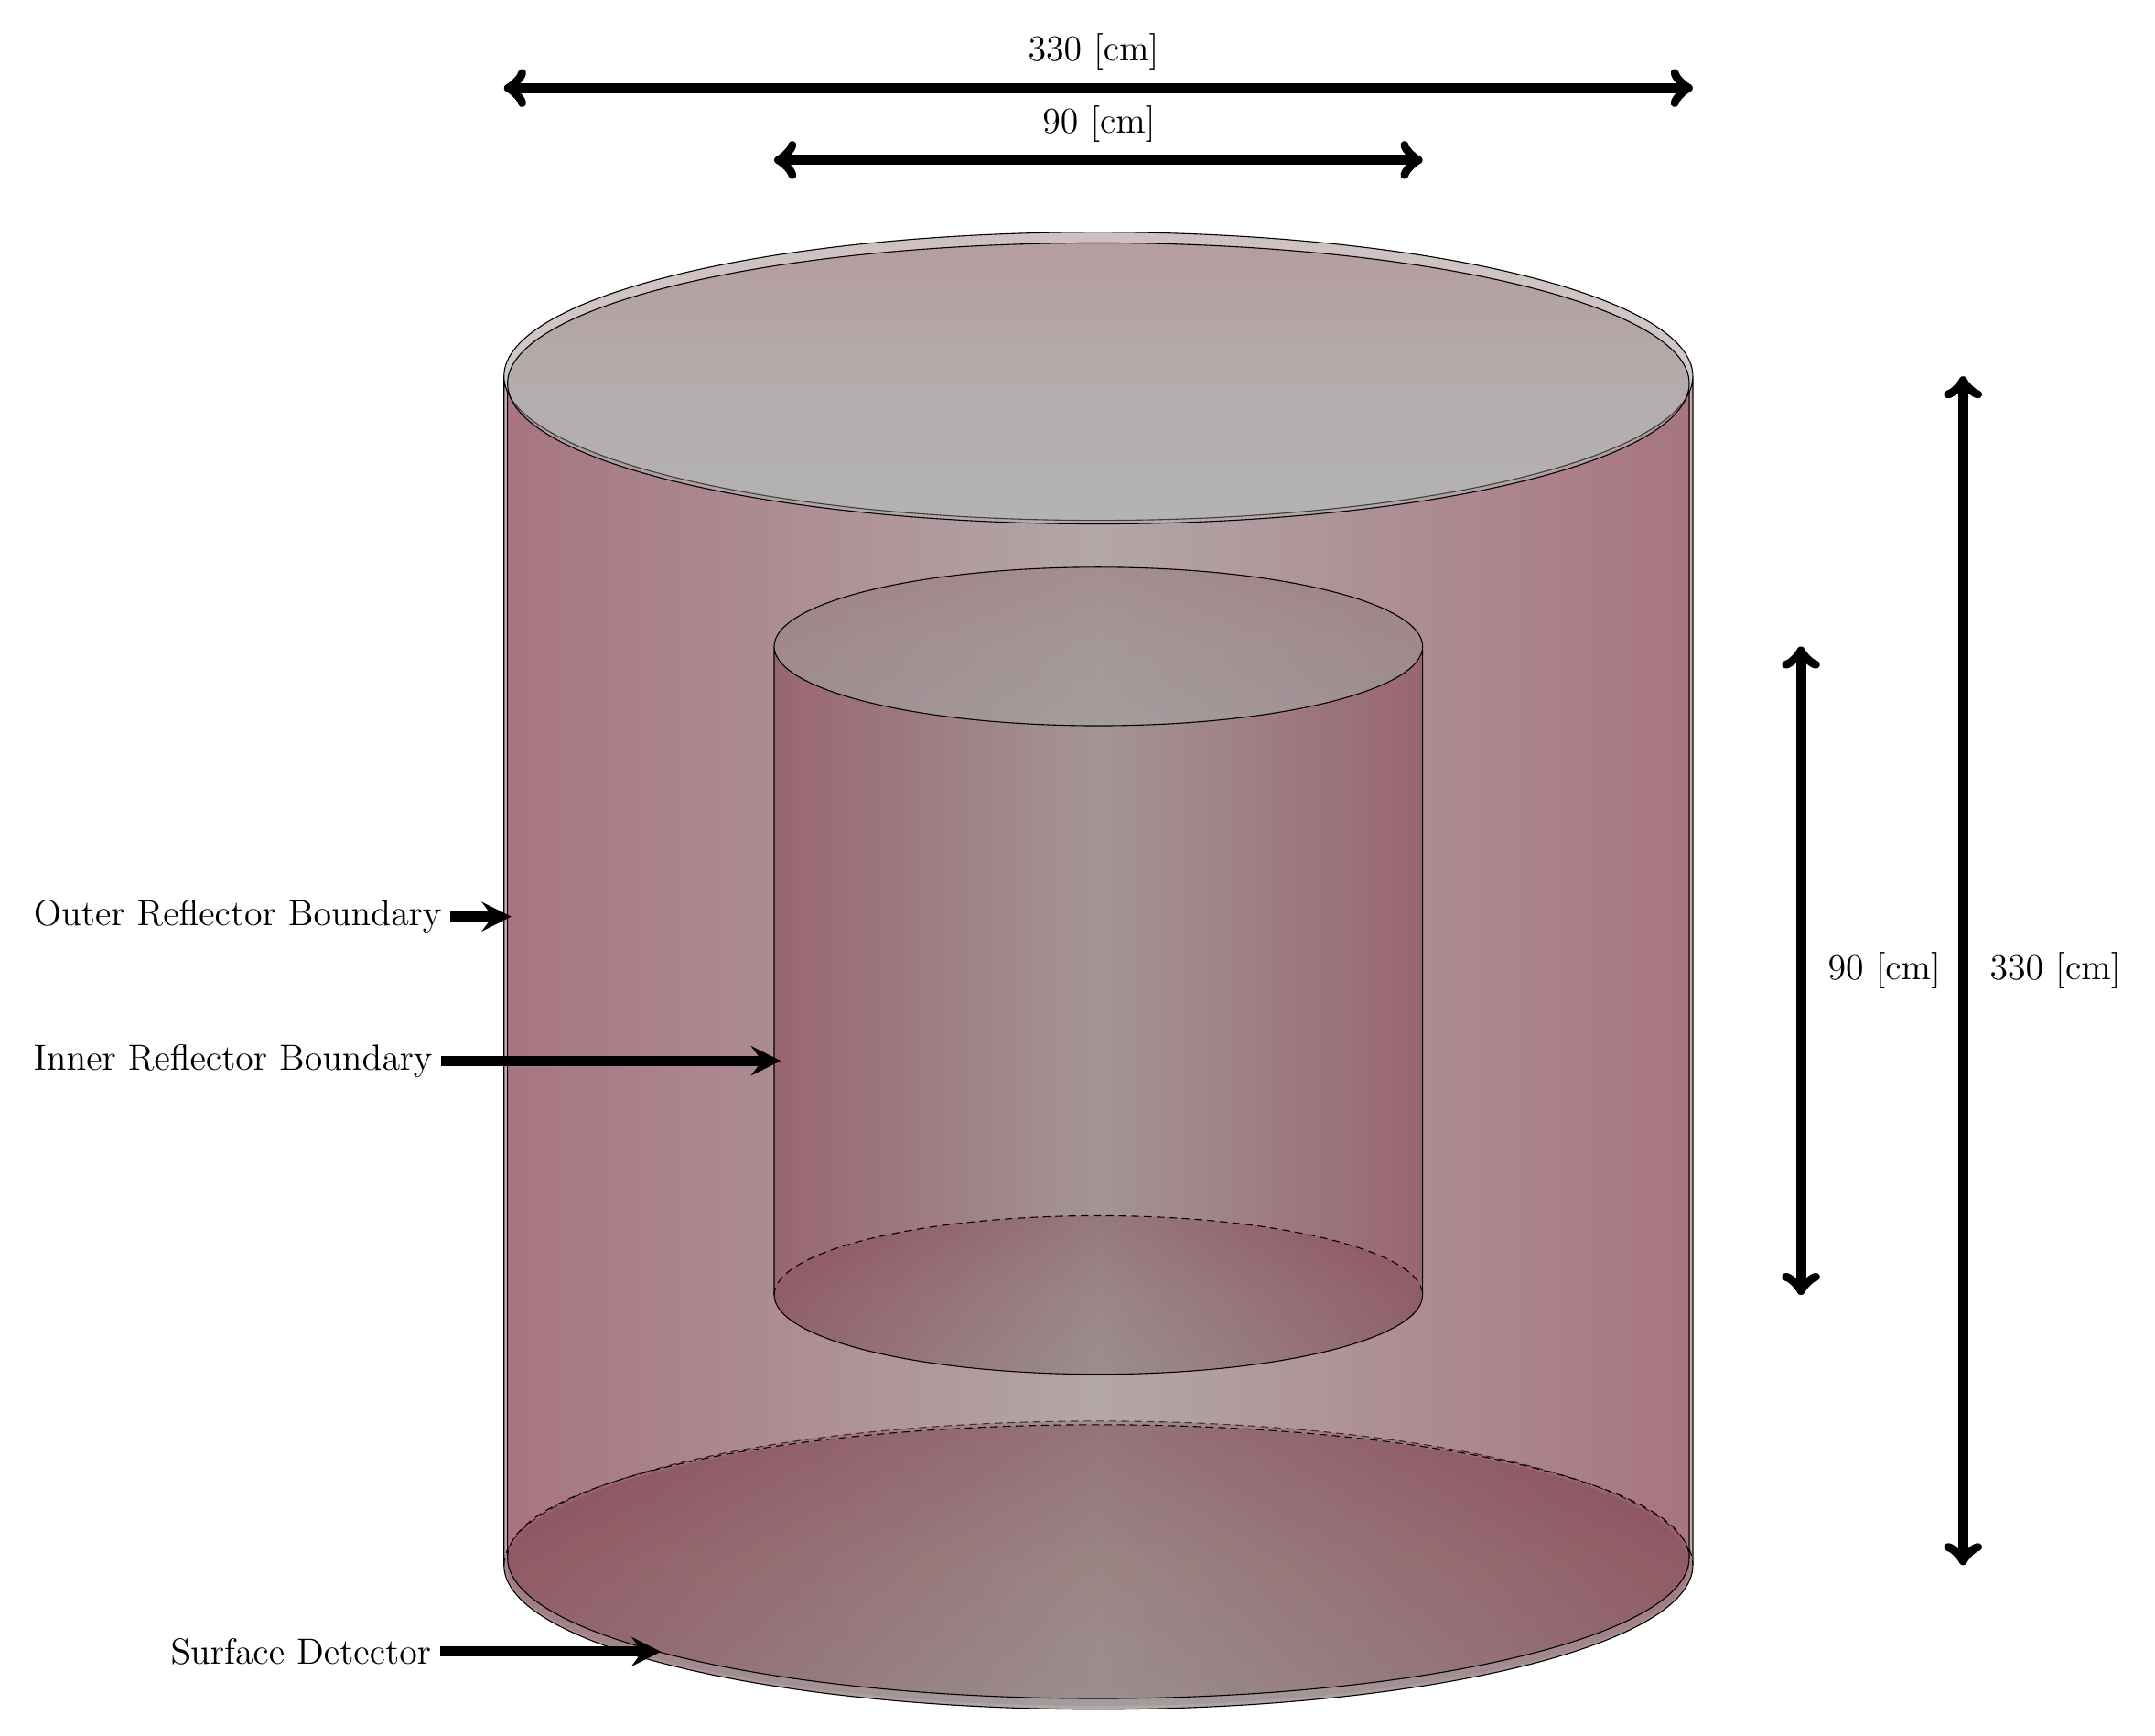
\begin{tikzpicture}
\fill[top color=pink!50!purple,bottom color=pink!10,middle color=pink,shading=axis,opacity=0.25] (0,0) circle (8.25cm and 2.0cm);
\fill[left color=pink!50!purple,right color=pink!50!purple,middle color=pink!50,shading=axis,opacity=0.25] (8.25,0) -- (8.25,16.5) arc (360:180:8.25cm and 2.0cm) -- (-8.25,0) arc (180:360:8.25cm and 2.0cm);
\fill[top color=pink!90!,bottom color=pink!2,middle color=pink!30,shading=axis,opacity=0.25] (0,16.5) circle (8.25cm and 2.0cm);
\draw (-8.25,16.5) -- (-8.25,0) arc (180:360:8.25cm and 2.0cm) -- (8.25,16.5) ++ (-8.25,0) circle (8.25cm and 2.0cm);
\draw[densely dashed] (-8.25,0) arc (180:0:8.25cm and 2.0cm);

\fill[top color=pink!50!purple,bottom color=pink!10,middle color=pink,shading=axis,opacity=0.25] (0,0.0) circle (8.2cm and 1.95cm);
\fill[left color=pink!50!purple,right color=pink!50!purple,middle color=pink!50,shading=axis,opacity=0.25] (8.2,0.1) -- (8.2,16.4) arc (360:180:8.2cm and 1.95cm) -- (-8.2,0.1) arc (180:360:8.2cm and 1.95cm);
\fill[top color=pink!90!,bottom color=pink!2,middle color=pink!30,shading=axis,opacity=0.25] (0,16.4) circle (8.2cm and 1.95cm);
\draw (-8.2,16.3) -- (-8.2,0.1) arc (180:360:8.2cm and 1.95cm) -- (8.2,16.3) ++ (-8.2,0.1) circle (8.2cm and 1.95cm);
\draw[densely dashed] (-8.2,0.1) arc (180:0:8.2cm and 1.85cm);

\fill[top color=pink!50!purple,bottom color=pink!10,middle color=pink,shading=axis,opacity=0.25] (0,3.75) circle (4.5cm and 1.1cm);
\fill[left color=pink!50!purple,right color=pink!50!purple,middle color=pink!50,shading=axis,opacity=0.25] (4.5,3.75) -- (4.5,12.75) arc (360:180:4.5cm and 1.1cm) -- (-4.5,3.75) arc (180:360:4.5cm and 1.1cm);
\fill[top color=pink!90!,bottom color=pink!2,middle color=pink!30,shading=axis,opacity=0.25] (0,12.75) circle (4.5cm and 1.1cm);
\draw (-4.5,12.75) -- (-4.5,3.75) arc (180:360:4.5cm and 1.1cm) -- (4.5,12.75) ++ (-4.5,3.75) (0,12.75) circle (4.5cm and 1.1cm);
\draw[densely dashed] (-4.5,3.75) arc (180:0:4.5cm and 1.1cm);

\node [anchor=west] (out-ref) at (-14.9, 9) {\Large Outer Reflector Boundary};
\node [anchor=west] (in-ref) at (-14.9, 7) {\Large Inner Reflector Boundary};
\node [anchor=west] (det) at (-13, -1.2) {\Large Surface Detector};

\draw [-stealth, line width=4pt, black] (out-ref) -- ++(3.8,0);
\draw [-stealth, line width=4pt, black] (in-ref) -- ++(7.6,0);
\draw [-stealth, line width=4pt, black] (det) -- ++(5.0,0);

\draw [-stealth, <->, line width=4pt, black] ++(-8.25,20.5) -- ++(16.5,0);
\draw [-stealth, <->, line width=4pt, black] ++(12,0) -- ++(0,16.5);

\node [anchor=west] (out-h) at (12.25, 8.25) {\Large 330 [cm]};
\node [anchor=west] (out-d) at (-1.1, 21.0) {\Large 330 [cm]};

\draw [-stealth, <->, line width=4pt, black] ++(-4.5,19.5) -- ++(9,0);
\draw [-stealth, <->, line width=4pt, black] ++(9.75,3.75) -- ++(0,9.0);

\node [anchor=west] (in-h) at (10.0, 8.25) {\Large 90 [cm]};
\node [anchor=west] (in-d) at (-0.9, 20.0) {\Large 90 [cm]};

\end{tikzpicture}
 }%
\caption{Detector Placement Inside Reflector in Sangamon200 and Sangamon20}
\label{fig:det-place}

\end{figure}


In Figure \ref{fig:det-place}, the graphite reflector outer boundary is shown, with the surface detector shell shown inside of it.  The active core region, which contains the fuel pebbles, is the innermost cylindrical region.  Its height is 2 $\left[cm\right]$ less than that of the reflector (e.g., the top of the detector is 1 $\left[cm\right]$ below the top of the reflector) and the radius is 1 $\left[cm\right]$ less than that of the reflector.  This detector measures the outward neutron current in $\left[\frac{neutrons}{s}\right]$.  To arrive at the unit of $\left[\frac{\#}{cm^2s}\right]$ most are familiar with, we divide by the detector's surface area thus:

\begin{align}
J^+ &= \frac{J_s^+ }{S_{d}}
\intertext{where}
J^+&= \mbox{ outward neutron current $\left[\frac{\#}{cm^2s}\right]$}\nonumber\\
J_s^+&= \mbox{ surface unadjusted outward neutron current $\left[\frac{\#}{s}\right]$}\nonumber\\
S_{d}&=\mbox{ detector surface area $[cm^2]$}\nonumber
\end{align}

After accounting for the surface area, the outward current at the detector in Sangamon200 is $9.156\times 10^{11} \pm 1.099\times 10^{09} \left[\frac{n}{cm^{2}s}\right]$.

\section{Sangamon20}
\label{s20}

Sangamon20 has identical material properties to Sangamon200, with the exception of the fuel, which is enriched to 19.75\% $^{235}U$ when fresh (and subsequently has a different isotopic composition as it burns).  It also assumes an identical power density, which is assumed not only in the single pebble models, but is also used when calculating the active core volume (see \autoref{r-h-vol}).  While the thermal power of Sangamon20 is 10\% that of Sangamon200, it isn't sufficient to simply scale Sangamon200's dimensions down to 10\% of their original values, as that wouldn't have the correct volume for the required pebbles, and the neutronics --- such as leakage --- would be inconsistent.  An inner core volume that is 10\% Sangamon200's should be a good approximation, but in order to be certain that this volume would hold the mass of fuel needed, a constraining calculation was carried out, which is detailed in \autoref{r-h-vol}.

\subsection{Graphite Reflector Thickness Determination}

As discussed in \autoref{s200}, the outward neutron current at the outer reflector boundary --- where the \acrshort{rpv} would be --- is used as the maximum acceptable value for outward neutron current in Sangamon20.  Figure \ref{fig:curr-v-ref} below provides the outward neutron current at the reflector boundary in Sangamon20 versus the thickness of the reflector.

\begin{figure}[h!]
\centering
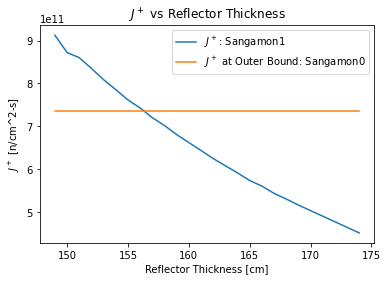
\includegraphics{figures/jout-v-rdet.png}
\caption{Outward Current vs Reflector Thickness}
\label{fig:jvrdet}
\end{figure}

Ultimately, the chosen reflector thickness was 75 $\left[ cm \right]$.

\subsection{Inner Core Volume Determination}
\label{r-h-vol}

The first assumption made in the scale-down is that Sangamon200 and Sangamon20 have the same specific power, or $\left[ \frac{\text{kW}}{\text{g UCO}} \right]$.

To calculate the mass of fuel in Sangamon200:


\begin{align}
M_{f,200} &= \frac{4}{3}\pi r_{u}^3 \rho_{u} n_{T} n_{p,200} \label{mf200}
\intertext{where}
M_{f,200}&= \mbox{ mass of fuel in Sangamon200 $\left[g\right]$}\nonumber\\
r_{u}&= \mbox{the radius of the UCO kernel inside a TRISO particle $\left[cm\right]$}\nonumber\\
\rho_{u}&= \mbox{ the density of UCO in $\left[\frac{g}{cc}\right]$}\nonumber\\
n_{T}&= \mbox{ number of TRISO particles in one pebble}\nonumber\\
n_{p}&= \mbox{ number of pebbles in Sangamon200}\nonumber
\end{align}


Using the parameters from Table \ref{table:params1}, the power density of Sangamon200 and Sangamon20 is 0.11 $[\frac{kW}{g}]$.  With a power capacity of 20 MWth, one can calculate the total mass of UCO in Sangamon20 as

\begin{align}
M_{f,20} &= \frac{P}{\rho_{p}} = 181818.18 \left[g\right]
\intertext{where}
M_{f,20}&= \mbox{ total mass of UCO in Sangamon20 [g]}\nonumber\\
P&= \mbox{ Thermal power of Sangamon20 [kW] }\nonumber\\
\rho_p &=\mbox{ Sangamon20's power density $[\frac{kW}{g}]$}\nonumber
\end{align}

Equation \ref{mf200} calculates the total mass of fuel in the Sangamon200 reactor by first calculating the mass of UCO in a single pebble using the density of UCO and the total volume of UCO kernels in a single pebble.  This value is then multiplied by the number of pebbles in Sangamon 200 (see Table \ref{table:params1}).  The total mass of fuel in the reactor divided by the mass of fuel in a single pebble gives the number of pebbles in the reactor, as follows:

\begin{align}
n_{p,20} &= \frac{M_{f,20}}{\frac{4}{3}r_{u}^3n_{T}\rho_{u}}
\intertext{where}
n_{p,20}&= \mbox{ number of pebbles in Sangamon20 [-]}\nonumber\\
M_{f,20}&= \mbox{ total mass of UCO in Sangamon20 [g]}\nonumber\\
r_u&=\mbox{ radius of a UCO kernel [cm]}\nonumber\\
n_{T}&= \mbox{ number of TRISO particles in a single pebble [-]}\nonumber\\
\rho_{u}&= \mbox{ density of UCO $[\frac{g}{cm^3}]$}\nonumber
\end{align}
\\
Rounding up - there can only be complete pebbles - we arrive at the number of pebbles for the Sangamon20 that are reported in Table \ref{table:params1}.

Knowing the number of pebbles is insufficient - the exact dimensions of the active core region are still undefined.  To determine the volume of this space, the formula uses concept of the packing fraction.  Assuming the pebble behavior is random loose packing \cite{tulluri_analysis_nodate} - the pebbles have unsystematically fallen into the core and the core is unshaken - the packing fraction in the range of 0.56 to 0.60 \cite{tulluri_analysis_nodate}.  Using the definitions above, the active core volume is

\begin{align}
V_{c,20} &= \frac{ n_{p,20}\frac{4}{3}\pi r_{p}^3 }{ \eta_{pf} }
\intertext{where}
V_{c,20}&= \mbox{ volume of the active core in Sangamon20 $[cm^2]$}\nonumber\\
n_{p,20}&= \mbox{ number of pebbles in Sangamon20 [-]}\nonumber\\
r_p&=\mbox{ radius of a pebble [cm]}\nonumber\\
\eta_{pf}&= \mbox{ packing fraction [-]}\nonumber
\end{align}

Using the formula for the volume of a cylinder, one can plot possible sets of $r_{c,20}$ and $h_{c,20}$ that satisfy the volume requirement, which is illustrated in \ref{fig:rh-vol}.

\begin{figure}[h!]
\centering
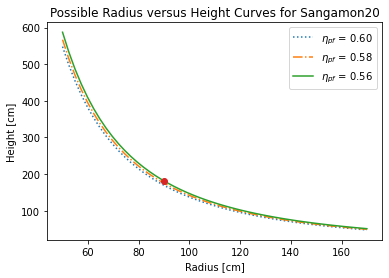
\includegraphics[width = 10cm]{figures/act-core-RH.png}
\caption{Curve of Possible Height and Radii by Packing Fraction}
\label{fig:rh-vol}
\end{figure}

The most critical configurations for a cylinder are either a \emph{square} shape, in which the height is equal to the diameter, or a \emph{flat} shape in which diameter is significantly greater than height.  As most designs use a height that is greater than or equal to the diameter, Sangamon20 is a square cylinder.  A packing fraction of 0.56 was ultimately chosen for Sangamon20 as it is the closest packing fraction to Sangamon200 while still staying in the range appropriate for haphazard packing.  The point indicated in \ref{fig:rh-vol} shows the radius and height selected for Sangamon20 - a radius of 90 $\left[cm\right]$, and a height of 180 $\left[cm\right]$.


\section{Heterogenization Tests}
\label{het-test-meth}

As described above, the pebbles use the approximation of a homogenized 'fueled-center', to reduce computational load.  This can, however, make the results of the simulation less accurate.  To determine the degree to which this affects reactor parameters such as $k_{eff}$ or outward neutron current, a few simulations performed undid this change, explicitly defining all TRISO particles in the pebbles, as they are in the single-pebble (infinite lattice) depletion models which generated the equilibrium fuel composition.  These so-called heterogenization tests compared the 2-group fast and thermal fluxes in the radial and axial direction.  In addition, they compared the lethargy-adjusted neutron energy spectrum using a 315-group energy structure.  Beyond showing the full spectra for each of these values for comparison, the relative difference is provided graphically for each so the differences induced by this change can be more readily observed.  Other than the choice to explicitly model the TRISO particles, the heterogenized model is identical to the Sangamon20 homogenized-pebble model.  The results of this test can be found in \autoref{res-hom}.

\section{Reactor Sensitivity to Pebble Locations and Symmetry}
\label{meth-sens}

By the nature of random pebble dispersal, there are a theoretically infinite number of perturbations to the Sangamon reactor models that are no different with the exception of slight variations in pebble locations.  It is also entirely possible to have bands in the reactor such that multiple pebbles of same (or similar) burnup align to form localized lines or pockets.  In the interest of better characterizing the extent to which these may effect the neutronics, we created a series of tests to explore the effect of various pebble composition locations.  

The \emph{shuffling} test maintained the pebble locations, but changed what composition the individual pebbles were (for results, see \autoref{res-shuff}).  As an example, Run 1 in the shuffle test makes all fresh, or "zero-pass" pebbles of the first-pass composition, first-pass pebbles of the second-pass, and so on down the line.  Run 2 makes the originally fresh (zero-pass) pebbles the second pass composition, the first-pass pebbles the third-pass composition, and so on. This scheme is described in \ref{table:shuffle}.

\begin{table}[h!]
\centering
\caption{Shuffle Test Run Schemes}
\begin{tabular}{ c  c  c  c  c  c  c }
 & \multicolumn{6}{c}{Position in Test Run} \\
\hline
Original Fuel Position in Control & Run 1 & Run 2 & Run 3 & Run 4 & Run 5 & Run 6  \\
\hline
0 & 1 & 2 & 3 & 4 & 5 & 6 \\
1 & 2 & 3 & 4 & 5 & 6 & 0 \\
2 & 3 & 4 & 5 & 6 & 0 & 1 \\
3 & 4 & 5 & 6 & 0 & 1 & 2 \\
4 & 5 & 6 & 0 & 1 & 2 & 3 \\
5 & 6 & 0 & 1 & 2 & 3 & 4 \\
6 & 0 & 1 & 2 & 3 & 4 & 5 \\
\hline
\end{tabular}

\label{table:shuffle}
\end{table}

The second analyzed the effects of utilizing a symmetry simplification, in order to improve computational speed (see \autoref{res-sym}) where $\frac{1}{6}$ of the core is modeled with a periodic boundary condition (neutrons exiting one side of the symmetry slice enter the other at the same height and trajectory).  We start with a full core model, and then select a slice from that core.  The slice used to simplify changed in each test, shown in Figure \ref{fig:slicetest}.  In each test, all other parameters remain the same.

\begin{figure}[h!]
\centering

\includegraphics[width=0.6\linewidth]{figures/run-layout.png}
\caption{Symmetry Test Run Layouts}
\label{fig:slicetest}
\end{figure}

In both tests, the $k_{eff}$ and outward currents are recorded and compared to the control model's $k_{eff}$ and $J^+$ (for results please refer to \autoref{res-control}).  A full spectrum of core components wasn't performed as in the heterogenous tests, as the difference between the results of this test and the control were small compared to the heterogeneity tests.  \autoref{app} and \autoref{app-sym} contains all geometry and mesh images for each run, and a pixel-by-pixel image difference of the mesh results.